%%%%%%%%%%%%%%%%%%%%%%%%%%%%%%%%%%%%%%%%%
% Beamer Presentation
% LaTeX Template
% Version 1.0 (10/11/12)
%
% This template has been downloaded from:
% http://www.LaTeXTemplates.com
%
% License:
% CC BY-NC-SA 3.0 (http://creativecommons.org/licenses/by-nc-sa/3.0/)
%
%%%%%%%%%%%%%%%%%%%%%%%%%%%%%%%%%%%%%%%%%

%----------------------------------------------------------------------------------------
%   PACKAGES AND THEMES
%----------------------------------------------------------------------------------------

\documentclass{beamer}

\mode<presentation> {

% The Beamer class comes with a number of default slide themes
% which change the colors and layouts of slides. Below this is a list
% of all the themes, uncomment each in turn to see what they look like.

%\usetheme{default}
%\usetheme{AnnArbor}
%\usetheme{Antibes}
%\usetheme{Bergen}
%\usetheme{Berkeley}
%\usetheme{Berlin}
%\usetheme{Boadilla}
%\usetheme{CambridgeUS}
%\usetheme{Copenhagen}
%\usetheme{Darmstadt}
%\usetheme{Dresden}
%\usetheme{Frankfurt}
%\usetheme{Goettingen}
%\usetheme{Hannover}
%\usetheme{Ilmenau}
%\usetheme{JuanLesPins}
\usetheme{Luebeck}
%\usetheme{Madrid}
%\usetheme{Malmoe}
%\usetheme{Marburg}
%\usetheme{Montpellier}
%\usetheme{PaloAlto}
%\usetheme{Pittsburgh}
%\usetheme{Rochester}
%\usetheme{Singapore}
%\usetheme{Szeged}
%\usetheme{Warsaw}

% As well as themes, the Beamer class has a number of color themes
% for any slide theme. Uncomment each of these in turn to see how it
% changes the colors of your current slide theme.

%\usecolortheme{albatross}
%\usecolortheme{beaver}
%\usecolortheme{beetle}
%\usecolortheme{crane}
%\usecolortheme{dolphin}
%\usecolortheme{dove}
%\usecolortheme{fly}
%\usecolortheme{lily}
%\usecolortheme{orchid}
%\usecolortheme{rose}
\usecolortheme{seagull}
%\usecolortheme{seahorse}
%\usecolortheme{whale}
%\usecolortheme{wolverine}

%\setbeamertemplate{footline} % To remove the footer line in all slides uncomment this line
%\setbeamertemplate{footline}[page number] % To replace the footer line in all slides with a simple slide count uncomment this line

%\setbeamertemplate{navigation symbols}{} % To remove the navigation symbols from the bottom of all slides uncomment this line
}

\usepackage{graphicx} % Allows including images
\usepackage{booktabs} % Allows the use of \toprule, \midrule and \bottomrule in tables

%----------------------------------------------------------------------------------------
%   TITLE PAGE
%----------------------------------------------------------------------------------------

\title[Vim Intro]{Comprehensive introduction to Vim} % The short title appears at the bottom of every slide, the full title is only on the title page

\author{Aleksander Gajewski} % Your name
\institute[None] % Your institution as it will appear on the bottom of every slide, may be shorthand to save space
{
\textit{aleksander@gajewski.fr} % Your email address
}
\date{\today} % Date, can be changed to a custom date

\begin{document}

\begin{frame}
\titlepage % Print the title page as the first slide
\end{frame}

\begin{frame}
  \frametitle{Overview}
  Vim is a highly customizable, modal editor. It is extensible with built-in vimscript language, python-support and huge collection of plugins.\\
  This presentation is intended to give a general overview of Vim and be a first reference for a novice user to start using its feature efficiently.\\
  For futher information please:
  \begin{enumerate} 
    \item - use vim internal help (:h *topic*)
    \item - run vimtutor
    \item - visit vimcasts.org
    \item - visit learnvimscriptinahardway.com
  \end{enumerate}
\end{frame}

\begin{frame}[fragile]
\frametitle{Vi Improved}
 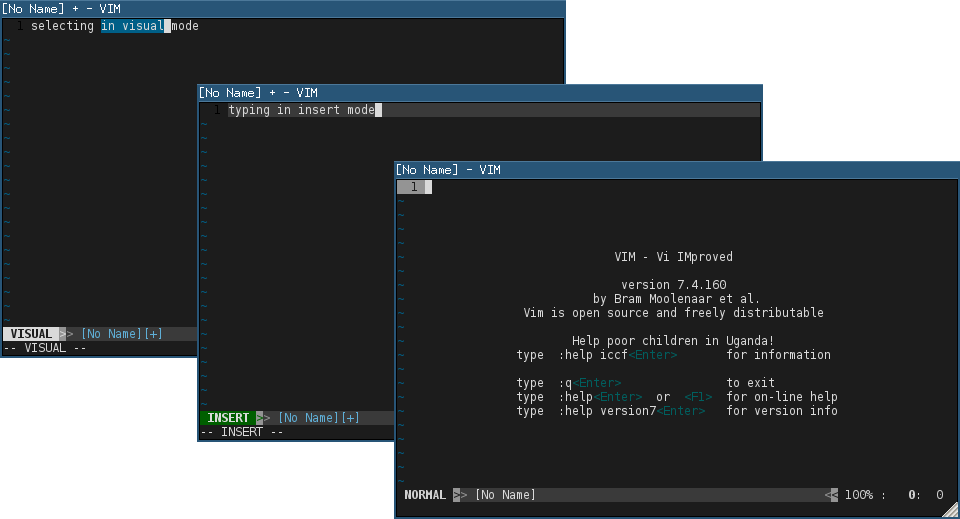
\includegraphics[width=\textwidth]{vim_screen.png}
\end{frame}

\begin{frame}[fragile]
  \frametitle{Modes overview *vim-modes*}
  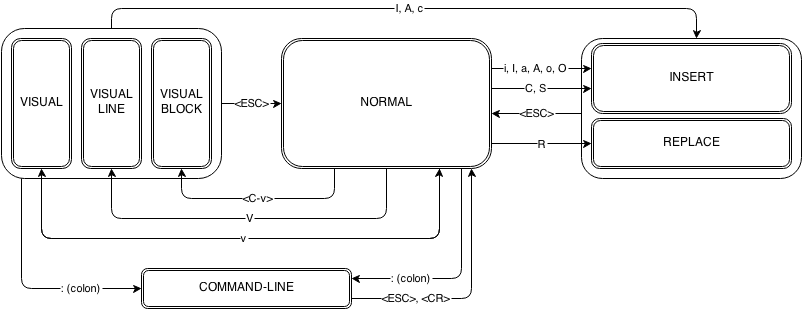
\includegraphics[width=\textwidth]{vim_modes.png}
\end{frame}

\begin{frame}
  \frametitle{Load/Save/Quit}
  Basic commands:
  \begin{enumerate}
    \item :e filename - edit/reload file
    \item :w - save file
    \item :q (:q!) - quit (without saving)
    \item :wq - save and quit
    \item :sav filename - 'save as' file (and open in current window)
  \end{enumerate}

  Useful ones:
  \begin{enumerate}
    \item :[range]w filename - write range to file
    \item :r filename - insert file below the cursor
  \end{enumerate}
\end{frame}

\begin{frame}
  \frametitle{Moving around}
  There is a huge boost while not using arrow keys to moving.
  \begin{enumerate}
    \item h (left), j (down), k (up), l (right) \\
    \item gg (begin of file), G (end of file) \\
    \item :<linenumber> - go to line
  \end{enumerate}
  All motion will be precisely described on further slides.
\end{frame}

\begin{frame}
  \frametitle{Buffers / Windows / Tabs}
  Summary:
  \begin{enumerate}
    \item A buffer is the in-memory text of a file.
    \item A window is a viewport on a buffer.
    \item A tab page is a collection of windows.
  \end{enumerate}
\end{frame}

\begin{frame}
  \frametitle{Buffers / Windows / Tabs: topics}
  \begin{itemize} 
    \item *opening-window* (new, split, vsplit) \\
    \item *window-move-cursor* \\
    \item
      \begin{enumerate}
        \item C-w jhlk
        \item C-w C-w
      \end{enumerate}
    \item *window-moving* \\
    \item *window-resize* \\
    \item *buffer-list* \\
    \item *list-repeat* (:bufdo, :windo, :tabdo)
  \end{itemize}
\end{frame}

\begin{frame}
  \frametitle{Copying and Moving Text}

  \begin{enumerate}
    \item "\{a-zA-Z0-9\}    Use register \{a-zA-Z0-9\} for next delete, yank or put (use uppercase character to append with delete and yank)
    \item :reg[isters]  Display the contents of all registers.
    \item \["x\]y\{motion\}   Yank \{motion\} text [into register x].
    \item \["x\]yy    Yank [count] lines [into register x]
    \item \["x\]Y     yank [count] lines [into register x] (synonym for yy).
    \item \{Visual\}["x]y   Yank the highlighted text [into register x] (for \{Visual\} see Selecting Text).
    \item \{Visual\}["x]Y   Yank the highlighted lines [into register x]
    \item :[range]y[ank] [x]    Yank [range] lines [into register x].
    \item :[range]y[ank] [x] \{count\}  Yank \{count\} lines, starting with last line number in [range] (default: current line), [into register x].
    \item ["x]p, ["x]P      Put the text [from register x] after (for P before) the cursor [count] times.
    \item ["x]gp, ["x]gP    Just like "p" ("P"), but leave the cursor just after the new text.
    \item :[line]pu[t] [x], :[line]pu[t]! [x]   Put the text [from register x] after (before) [line] (default current line).
  \end{enumerate}
\end{frame}

\begin{frame}
  \frametitle{Undo/Redo/Repeat}

  \begin{enumerate}
    \item [count]u     Undo [count] changes.
    \item :u[ndo]   Undo one change.
    \item [count]CTRL-R    Redo [count] changes which were undone.
    \item :red[o]   Redo one change which was undone.
    \item U     Undo all latest changes on one line.
    \item .     Repeat last change, with count replaced with [count].
  \end{enumerate}
\end{frame}

\begin{frame}
  \frametitle{operator \& motions}
  \begin{enumerate}
    \item c change
    \item d delete
    \item y yank into register (does not change the text)
    \item gu make lowercase
    \item gU make uppercase
    \item ! filter through an external program
    \item = filter through equalprg or C-indenting if empty
    \item gq text formatting
    \item g? ROT13 encoding
    \item zf    define a fold
  \end{enumerate}
\end{frame}

\begin{frame}
  \frametitle{2. Left-right motions                 *left-right-motions*}

  \begin{enumerate}
    \item h, <Left>, CTRL-H, <BS>           [count] characters to the left.
    \item l, <Right>, <Space>           [count] characters to the right.
    \item 0         To the first character of the line.
    \item <Home>            To the first character of the line.
    \item f\{char\}         To [count]th occurrence of \{char\} to the right.  The
    \item           cursor is placed on \{char\} inclusive
    \item F\{char\}         To the [count]'th occurrence of \{char\} to the left.
    \item           The cursor is placed on \{char\} exclusive.
    \item t\{char\}         Till before [count]'th occurrence of \{char\} to the
      right.  The cursor is placed on the character left of
      \{char\} |inclusive|.
    \item T\{char\}         Till after [count]'th occurrence of \{char\} to the left.  The cursor is placed on the character right of \{char\} exclusive.
    \item ;         Repeat latest f, t, F or T [count] times.
    \item ,         Repeat latest f, t, F or T in opposite direction [count] times.
  \end{enumerate}
\end{frame}

\begin{frame}
  \frametitle{3. Up-down motions                    *up-down-motions*}
  k, <Up>, CTRL-P           [count] lines upward |linewise|.
  j, <Down>, CTRL-J

  CTRL-N            [count] lines downward |linewise|.

  gk, g<Up>         [count] display lines upward.  |exclusive| motion.
  Differs from 'k' when lines wrap, and when used with
  an operator, because it's not linewise.  \{not in Vi\}

  gj, g<Down>           [count] display lines downward.  |exclusive| motion.
  G         Goto line [count], default last line, on the first
  non-blank character |linewise|.  If 'startofline' not
  set, keep the same column.
  G is a one of |jump-motions|.
  <C-End>           Goto line [count], default last line, on the last character |inclusive|. \{not in Vi\}
  <C-Home>, gg          Goto line [count], default first line, on the first non-blank character |linewise|.  If 'startofline' not set, keep the same column.
  :[range]      Set the cursor on the last line number in [range].
  [range] can also be just one line number, e.g., ":1"
  or ":'m".
  In contrast with |G| this command does not modify the
  |jumplist|.
  *N%*
  \{count\}     Go to \{count\} percentage in the file, on the first
  non-blank in the line |linewise|.  To compute the new
  line number this formula is used:
  (\{count\} * number-of-lines + 99) / 100
  See also 'startofline' option.  \{not in Vi\}
\end{frame}

\begin{frame}
  \frametitle{4. Word motions                       *word-motions*}
  w         [count] words forward.  |exclusive| motion.
  <C-Right> or                  *<C-Right>* *W*
  W         [count] WORDS forward.  |exclusive| motion.
  e         Forward to the end of word [count] |inclusive|.
  Does not stop in an empty line.
  E         Forward to the end of WORD [count] |inclusive|.
  Does not stop in an empty line.
  <S-Left>  or                  *<S-Left>* *b*
  b         [count] words backward.  |exclusive| motion.
  <C-Left>  or                  *<C-Left>* *B*
  B         [count] WORDS backward.  |exclusive| motion.
  ge            Backward to the end of word [count] |inclusive|.
  gE            Backward to the end of WORD [count] |inclusive|.
\end{frame}

\begin{frame}
  \frametitle{5. Text object motions                    *object-motions*}
  (         [count] sentences backward.  |exclusive| motion.
  )         [count] sentences forward.  |exclusive| motion.
  \{            [count] paragraphs backward.  |exclusive| motion.
  \}            [count] paragraphs forward.  |exclusive| motion.
]]          [count] sections forward or to the next '\{' in the
  first column.  When used after an operator, then also
stops below a '\}' in the first column.  |exclusive|
Note that |exclusive-linewise| often applies.
][          [count] sections forward or to the next '\}' in the
first column.  |exclusive|
Note that |exclusive-linewise| often applies.
[[          [count] sections backward or to the previous '\{' in
      the first column.  |exclusive|
      Note that |exclusive-linewise| often applies.
    []          [count] sections backward or to the previous '\}' in
    the first column.  |exclusive|
    Note that |exclusive-linewise| often applies.
\end{frame}

\begin{frame}
    \frametitle{6. Text object selection            *object-select* *text-objects*}
    yaw         "a word", select [count] words (see |word|).
    Leading or trailing white space is included, but not
    counted.
    When used in Visual linewise mode "aw" switches to
    Visual characterwise mode.
    iw          "inner word", select [count] words (see |word|).
    White space between words is counted too.
    When used in Visual linewise mode "iw" switches to
    Visual characterwise mode.
    aW          "a WORD", select [count] WORDs (see |WORD|).
    Leading or trailing white space is included, but not
    counted.
    When used in Visual linewise mode "aW" switches to
    Visual characterwise mode.
    iW          "inner WORD", select [count] WORDs (see |WORD|).
    White space between words is counted too.
    When used in Visual linewise mode "iW" switches to
    Visual characterwise mode.
    as          "a sentence", select [count] sentences (see
    |sentence|).
    When used in Visual mode it is made characterwise.
    is          "inner sentence", select [count] sentences (see
    |sentence|).
    When used in Visual mode it is made characterwise.
    ap          "a paragraph", select [count] paragraphs (see
    |paragraph|).
    Exception: a blank line (only containing white space)
    is also a paragraph boundary.
    When used in Visual mode it is made linewise.
    ip          "inner paragraph", select [count] paragraphs (see
    |paragraph|).
    Exception: a blank line (only containing white space)
    is also a paragraph boundary.
    When used in Visual mode it is made linewise.
a]                      *v\_a]* *v\_a[* *a]* *a[*
  a[            "a [] block", select [count] '[' ']' blocks.  This
    goes backwards to the [count] unclosed '[', and finds
    the matching ']'.  The enclosed text is selected,
    including the '[' and ']'.
    When used in Visual mode it is made characterwise.
i]                      *v\_i]* *v\_i[* *i]* *i[*
  i[            "inner [] block", select [count] '[' ']' blocks.  This
    goes backwards to the [count] unclosed '[', and finds
    the matching ']'.  The enclosed text is selected,
    excluding the '[' and ']'.
    When used in Visual mode it is made characterwise.
    a)                          *v\_a)* *a)* *a(*
    a(                          *v\_ab* *v\_a(* *ab*
    ab          "a block", select [count] blocks, from "[count] [(" to
      the matching ')', including the '(' and ')' (see
      |[(|).  Does not include white space outside of the
        parenthesis.
        When used in Visual mode it is made characterwise.

        i) i(   ib          "inner block", select [count] blocks, from "[count] [("
          to the matching ')', excluding the '(' and ')' (see
          |[(|).
            When used in Visual mode it is made characterwise.
            a>, a<          "a <> block", select [count] <> blocks, from the
            [count]'th unmatched '<' backwards to the matching
            '>', including the '<' and '>'.
            When used in Visual mode it is made characterwise.

            i<, i<          "inner <> block", select [count] <> blocks, from
            the [count]'th unmatched '<' backwards to the matching
            '>', excluding the '<' and '>'.
            When used in Visual mode it is made characterwise.
            at          "a tag block", select [count] tag blocks, from the
            [count]'th unmatched "<aaa>" backwards to the matching
            "</aaa>", including the "<aaa>" and "</aaa>".
            See |tag-blocks| about the details.
            When used in Visual mode it is made characterwise.
            it          "inner tag block", select [count] tag blocks, from the
            [count]'th unmatched "<aaa>" backwards to the matching
            "</aaa>", excluding the "<aaa>" and "</aaa>".
            See |tag-blocks| about the details.
            When used in Visual mode it is made characterwise.

          a\} a\{   aB          "a Block", select [count] Blocks, from "[count] [\{" to
              the matching '\}', including the '\{' and '\}' (see
              |[\{|).
                  When used in Visual mode it is made characterwise.

                i\}         i\{ iB          "inner Block", select [count] Blocks, from "[count] [\{"
                    to the matching '\}', excluding the '\{' and '\}' (see
                    |[\{|).
                        When used in Visual mode it is made characterwise.

                        a" a'   a`                          *v\_a`* *a`*
                        "a quoted string".  Selects the text from the previous
                        quote until the next quote.  The 'quoteescape' option
                        is used to skip escaped quotes.
                        Only works within one line.
                        When the cursor starts on a quote, Vim will figure out
                        which quote pairs form a string by searching from the
                        start of the line.
                        Any trailing white space is included, unless there is
                        none, then leading white space is included.
                        When used in Visual mode it is made characterwise.
                        Repeating this object in Visual mode another string is
                        included.  A count is currently not used.

                        i" i'   i
                        Like a", a' and a`, but exclude the quotes and
                        repeating won't extend the Visual selection.
                        Special case: With a count of 2 the quotes are
                        included, but no extra white space as with a"/a'/a`.


                      \end{frame}

\begin{frame}[fragile]
  \frametitle{7. Marks                  *mark-motions* *}

                        \begin{verbatim}
                        Jumping to a mark can be done in two ways:
                        1. With ` (backtick):     The cursor is positioned at the specified location
        and the motion is |exclusive|.
        2. With '' (single quote): The cursor is positioned on the first non-blank
        character in the line of the specified location and
        the motion is linewise.


            *m* *mark* *Mark*
            m\{a-zA-Z\}     Set mark \{a-zA-Z\} at cursor position (does not move
      the cursor, this is not a motion command).

      '\{a-z\}  `\{a-z\}        Jump to the mark \{a-z\} in the current buffer.


            *'A* *'0* *`A* *`0*
            '\{A-Z0-9\}  `\{A-Z0-9\}    To the mark \{A-Z0-9\} in the file where it was set (not
      a motion command when in another file).  \{not in Vi\}
      marks 
      :reg[isters] \{arg\}  Display the contents of the numbered and named
      registers that are mentioned in \{arg\}.  For example:
        :dis 1a
      to display registers '1' and 'a'.  Spaces are allowed
      in \{arg\}.  \{not in Vi\}
      :di[splay] [arg]  Same as :registers.  \{not in Vi\}
      ["x]y\{motion\}       Yank \{motion\} text [into register x].  When no
      characters are to be yanked (e.g., "y0" in column 1),
      this is an error when 'cpoptions' includes the 'E'
      flag.
      ["x]yy            Yank [count] lines [into register x] |linewise|.
      ["x]Y         yank [count] lines [into register x] (synonym for
      yy, |linewise|).  If you like "Y" to work from the
      cursor to the end of line (which is more logical,
      but not Vi-compatible) use ":map Y y\$".
      \{Visual\}["x]y       Yank the highlighted text [into register x] (for
      \{Visual\} see |Visual-mode|).  \{not in Vi\}
      \{Visual\}["x]Y       Yank the highlighted lines [into register x] (for
      \{Visual\} see |Visual-mode|).  \{not in Vi\}
      :[range]y[ank] [x]    Yank [range] lines [into register x].
      :[range]y[ank] [x] \{count\}
      Yank \{count\} lines, starting with last line number
      in [range] (default: current line |cmdline-ranges|),
      [into register x].
      ["x]p         Put the text [from register x] after the cursor
      [count] times.  \{Vi: no count\}
      ["x]P         Put the text [from register x] before the cursor
      [count] times.  \{Vi: no count\}
      ["x]<MiddleMouse> Put the text from a register before the cursor [count]
      times.  Uses the "* register, unless another is
      specified.
      Leaves the cursor at the end of the new text.
      Using the mouse only works when 'mouse' contains 'n'
      or 'a'.
      \{not in Vi\}
      If you have a scrollwheel and often accidentally paste
      text, you can use these mappings to disable the
      pasting with the middle mouse button:
        :map <MiddleMouse> <Nop>
        :imap <MiddleMouse> <Nop>
      You might want to disable the multi-click versions
      too, see |double-click|.
      ["x]gp            Just like "p", but leave the cursor just after the new
      text.  \{not in Vi\}
      ["x]gP            Just like "P", but leave the cursor just after the new
      text.  \{not in Vi\}
  \end{verbatim}
\end{frame}

\begin{frame}
  \frametitle{registers}

  \begin{enumerate}
    \item "\{a-zA-Z0-9\}    Use register \{a-zA-Z0-9\} for next delete, yank or put (use uppercase character to append with delete and yank)
    \item :reg[isters]
  \end{enumerate}
\end{frame}

\begin{frame}
  \frametitle{macros}
  \begin{enumerate}
    \item qd    start recording to register d
    \item ...   your complex series of commands
    \item q     stop recording
    \item @d    execute your macro
    \item @@    execute your macro again
    \item :g/pattern/normal @q
  \end{enumerate}
\end{frame}

\begin{frame}
  \frametitle{vimdiff}
  \begin{enumerate}
    \item vimdiff file1 file2
    \item :diffthis :sp file2 :diffthis
    \item :diffoff
    \item [c ]c
    \item rangediffget
    \item rangediffput
  \end{enumerate}
\end{frame}

\begin{frame}
  \frametitle{substitutions}
      %  \\( \\) . * + [^ ]
      %  \& \1 \2
      g c
      =
      usage of * \#
      nohl
      \= call foo()
      \= substitute
      submatch()

let g:I=1
%g/^- id: \d\+$/ s/\d\+/\=g:I/|let g:I=g:I+1

%:.+1,$g/^- id: \d\+$/normal! 0^A

\end{frame}

\begin{frame}
  \frametitle{Command mode}
  working with ctrl+r
\end{frame}


\section{PLUGINS}
\begin{frame}
  \frametitle{nerdtree, vim-nerdtree-tab}
  Navigate through filesystem.
  Allows open, open split h/v, open tab, quick preview.
  Support for bookmarks.
  :NERDTreeFind
  plugin nerdtree-tabs keeps nerd tree toggle accross all tabs
\end{frame}

\begin{frame}
  \frametitle{tagbar}
  outline with tags, variables, classes, function
\end{frame}

\begin{frame}
  \frametitle{undotree}
  visualize (with diff) and navigate through the history of file changel
\end{frame}

\begin{frame}
  \frametitle{fugitive}
  git facilities
\end{frame}

\begin{frame}
  \frametitle{tabular}

\end{frame}

\begin{frame}
  \frametitle{airline}
\end{frame}

\begin{frame}
  \frametitle{vim-slime}
\end{frame}


\begin{frame}
  \frametitle{abolish}
\end{frame}

\begin{frame}
  \frametitle{abbreviations / and hideing}
      iab
      conceal demo
      %if has('conceal')
      %  " may be adgms
      %  let g:tex\_conceal="adgm"
      %  set conceallevel=2
      %  highlight! link Conceal texMathSymbol
      %endif
      %syn match texMathSymbol '\\alpha\>' contained conceal cchar=α
      %syn match texMathSymbol '\\beta\>' contained conceal cchar=β
      %syn match texMathSymbol '\\gamma\>' contained conceal cchar=γ
\end{frame}

\begin{frame}
  \frametitle{expressions register}
  <C-r>=<C-r>"<CR>
\end{frame}

\begin{frame}
  \frametitle{colorschemes / cursorcolumn line / hexhighlight}
\end{frame}

\begin{frame}
  \frametitle{spell check}
      :setlocal spell spelllang=en\_us
    ]s          Move to next misspelled word after the cursor.
    A count before the command can be used to repeat.
    'wrapscan' applies.
    [s          Like "]s" but search backwards, find the misspelled
    word before the cursor.  Doesn't recognize words
    split over two lines, thus may stop at words that are
    not highlighted as bad.  Does not stop at word with
    missing capital at the start of a line.
    z=          For the word under/after the cursor suggest correctly
    spelled words.  This also works to find alternatives
    for a word that is not highlighted as a bad word,
    e.g., when the word after it is bad.
\end{frame}

\begin{frame}
    \frametitle{folds}
    zf{motion}, {Visual}zf  Operator to create a fold.  This only works when 'foldmethod' is "manual" or "marker".  The new fold will be closed for the "manual" method.  'foldenable' will be set.
    :{range}fo[ld]   Create a fold for the lines in {range}.  Works like "zf".
    zd      Delete one fold at the cursor.
    zo      Open one fold under the cursor.
    zO      Open all folds under the cursor recursively.
    zc      Close one fold under the cursor.
    zC      Close all folds under the cursor recursively.
\end{frame}

\begin{frame}
  \frametitle{Other features}
  list number
    built in autocomplete / no prob with connecting external tools
    topics to cover:
    context autocomplete
    inplace static source code analyser
    CA CX CxCf CE CY
\end{frame}

\begin{frame}
    vimrc / recommended setup / mappings vimscript basic (function declaration / scopes / if / types / )
    (sort)
    os interaction (in place edit)
    external indent
    vimcasts.org
    vimgolf.org
    http://learnvimscriptthehardway.stevelosh.com/
\end{frame}

\end{document}

